%Linea Para poder completar automaticamente las citas con el Sublime
%No hace el documento, se puede borrar esta linea si no se usa el Sublime
%------------------------------------------------------------------------------
 \newcommand{\NoBiblioMicro}[1]{
 \ifthenelse{\equal{#1}{verdadero}}{}{\bibliography{Referencias/base_bibliografica}}
 \NoBiblioMicro{verdadero}}
 %-----------------------------------------------------------------------------

%Formato (Nombre de capitulo largo o corto), nombre del capitulo, resumen y estilo de la
%Portada del Capitulo
%------------------------------------------------------------------------------
 
 %Formato en si, titulo en dos renglones
 \FormatoCapituloDosLineas
 
 %Nombre y etiquete para referir
 \chapter{Microfabricación de los electrodos}\label{chap:Microfabricacion}

 %Para que no salga el numero de pagina en la portada del capitulo
 \thispagestyle{empty}
	
 %Resumen del Capitulo en Italica
 \noindent\textit{En este capítulo se describen los resultados obtenidos durante en la fabricación de electrodos recubiertos con películas delgadas mesoporosas de SiO$_2$ o Si$_x$Zr$_{1-x}$O$_2$. Se analizan los diseños utilizados, los materiales empleados, las técnicas aplicadas y las caracterizaciones llevadas a cabo. Principalmente se evaluó el desempeño electroquímico\index{electroquimico} de los electrodos por un lado, y la compatibilidad con las síntesis sol-gel\index{sol-gel} por otro, de forma de compatibilizar los procesos \textit{top-down }con los \textit{bottom-up.}. Por último se presentan los resultados EQ  para sonda\index{sonda}s modelos (\fe, \ru\space y \fc)obtenidos con un prototipo de sensor\index{sensor} compuestos por electrodos recubiertos con distintas películas.}\index{bottom-up@\textit{bottom-up}}\index{top-down@\textit{top-down}}
 
 
 %Indice de capitulo alineada al borde inferior de la pagina, nueva pagina
 \vfill
 \minitoc
 \newpage
 %-------------------------------------------------------------------------------

\section{Introducción}
	
	El diseño y desarrollo de un multisensor electroquímico\index{electroquimico} selectivo, integrado y escalable basado en \pdm\space consta de dos bloques constructivos fundamentales: las películas delgadas mesoporosas y los electrodos. En el capítulo \ref{chap:Mesoporosos}, se discutió y analizó la elección de los materiales para conformar la película delgada \index{película!delgada}mesoporososa con la cual se recubren los electrodos. En el capítulo \ref{chap:Electroquimica} se realizó un estudio profundo las propiedades de transporte, la capacidad de preconcentrar, excluir y estabilidad química de dichos recubrimientos sobre películas delgadas de Au.

	La integración de los procesos \textit{bottom-up}\index{bottom-up@\textit{bottom-up}}, propios de procesos de síntesis químicas, y \textit{top-down}\index{top-down@\textit{top-down}}, aquellos usados en microfabricación\index{microfabricación}, nunca es trivial. El sólo hecho de depositar soles\index{sol} con precursor\index{precursor}es de óxidos sobre oro, que resulten en películas delgadas homogéneas, bien adheridas sin grietas ni fisuras, ya es un desafío, como se vió en el capítulo \ref{chap:Mesoporosos}. El objetivo, luego de desarrollar los métodos a bajas temperaturas para la síntesis de \pdm, de optimizar y estudiar su estructura y de comprender los procesos de transporte\index{transporte} a través de las películas, es poder depositarlos sobre estructuras de oro\index{oro} con un diseño optimizado para usarlo como sensor. 

	El depósito\index{depósito} de soles\index{sol} sobre una superficie\index{superficie} que tenga dos o más capas de distintos  materiales trae asociadas dificultades inherentes a las propiedades físicas y químicas de cada uno de ellas. Pueden diferir en el coeficiente de expansión térmica, en la química superficial, en la afinidad por el H$_2$O o solventes, etc.
	Es por ello que el diseño debe considerar los materiales que se usarán y sus propiedades, así como racionalizar la estructura de los electrodos considerando resistencia eléctrica, espesor\index{espesor} de los electrodos y facilidad para la fabricación. También es fundamental tener en cuenta una serie de factores a la hora de imprimir las máscara\index{máscara}s para los sensores. Principalmente la resolución de línea que se puede obtener según el tipo de máscara\index{máscara}, cantidad de electrodos de trabajo\index{electrodo!de trabajo} por sensor, calcular el área óptima para obtener señales aceptables, estimar resistencias, distancias entre electrodos y demás parámetros.

	El material para los electrodos también se debe elegir cuidadosamente. Se trata de un compromiso entre tres factores: 1) compatibilidad con el óxido de las películas mesoporosas, 2) obtención de una respuesta electroquímica\index{electroquimico} de calidad y, 3) la facilidad para depositarlos y transferir los diseños por litografía.

	En este trabajo se priorizó generar diseños compactos, miniaturizar los electrodos y optimizarlos para obtener respuestas electroquímica\index{electroquimico}s\index{electroquimico} de buen desempeño. El oro\index{oro} posee excelentes propiedades para llevar a cabo reacciones de oxido-reducción y obtener una respuestas confiables y repetibles. Si \index{silicio}bien el Au\index{oro} es el material óptimo para este tipo de mediciones, existen otros materiales más económicos y, en algunos casos mas fáciles de depositar (tintas de carbono, óxido de indio/estaño, carbono vítreo, etc.), sin embargo, su respuesta electroquímica\index{electroquimico} es poco repetible, su rugosidad\index{rugosidad} es muy variable y tienen grandes desviaciones de la idealidad (sobre todo a altas velocidades de barrido).\cite{Wi2000,Villullas2000}

	En este capítulo se presentan los resultados colectados durante la fabricación de los microelectrodo\index{electrodo!microelectrodo}s. Se da cuenta de los diseños, se discuten las ventajas y desventajas de los procesos empleados y se pone énfasis en la compatibilidad con los métodos utilizados para el depósito\index{depósito} y condensación\index{condensación} de las \pdm\space realizados por procesos sol-gel\index{sol-gel}. Se evalúa la calidad de la transferencia del diseño, las dimensiones, la respuesta electroquímica\index{electroquimico} de los mismos y la posibilidad de escalar el proceso para producir sensores\index{sensor} electroquímico\index{electroquimico}s\index{electroquimico} basados en películas delgadas mesoporosas en cantidad.
	
\section{Microfabricación de los sensores}\label{sec:microfabricaci_n_de_los_sensores}
		
	 	 En las siguientes secciones se analizan los diseños de los sensores\index{sensor} y los resultados de la fabricación de los electrodos. Se discuten, también, las técnicas de microfabricación\index{microfabricación} empleadas y las caracterizaciones realizadas sobre los mismos. Por último, se analiza la compatibilidad con las técnicas sol-gel\index{sol-gel} para utilizarse como sustratos de películas delgadas mesoporosas.

  		\subsection{Consideraciones sobre el diseño}\label{sec:diseno}

			 Desde un principio surgió la idea de fabricar una plataforma con múltiples electrodos, de forma de tener sensores, para múltiples analitos, compactos y escalables. Para ello es importante proveer un diseño que tenga en cuenta los procesos que se usan en la industria electrón\index{electrón}ica, a fin de poder escalar el prototipo. Las siguientes secciones tratan esta temática; de qué manera se pueden generar diseños de electrodos para un sensor\index{sensor} multianalito, y cuales procesos pueden llevarse a cabo de forma de escalarlos y compatibilizar con los procesos de síntesis sol-gel\index{sol-gel}.

		 \subsubsection{Primer diseño}

		     El primer diseño contempló un sensor\index{sensor} con cuatro electrodos de trabajo\index{electrodo!de trabajo} (ET) y preveía utilizar contraelectrodo\index{electrodo!contraelectrodo} (CE) y electrodo de referencia\index{electrodo!de referencia} (ER) externos. 

		    	\begin{figure}[th!]
		 	       	\includegraphics[width=\textwidth]{Imagenes/diseno_mascara_v1.pdf}
 		       		\caption[Primer diseño y máscara\index{máscara} de los sensores]{Diseño y máscara\index{máscara} para la primera versión de los electrodos. A) diseño completo con 32 sensores\index{sensor} de 4 ET cada uno, B) Detalles de las marcas de alineación\index{marcas de alineación}, C) microscopía\index{microscopía} de la máscara\index{máscara} ya impresa donde se ven las imperfecciones de la impresión.}
 		         	\label{fig:diseno_mascara_v1}
 		     		\end{figure}
 		 	 \pagebreak
 		     		
		      Se trabajó con dimensiones relativamente grandes, con dos geometrías distintas, electrodos circulares con un radio R=\SI{300}{\um} y electrodos cuadrados de lado L=\SI{500}{\um}. Éste primer diseño, aunque simple y con un aprovechamiento del espacio poco eficiente cuenta con algunas ventajas destacadas. Resulta muy económico para la impresión de las máscara\index{máscara}s, áreas grandes de electrodos y pistas (para poder colocar fácilmente puntas de prueba y obtener valores altos de intensidad de modo de familiarizarse con las primeras respuestas EQ) y sencillo de fabricar debido a las dimensiones utilizadas.
		      % . Esto diseño sirvió para familiarizarse con las primeras mediciones EQ y sencillo de fabricar.  
		
		      La figura \ref{fig:diseno_mascara_v1} muestra el resultado de la impresión de este primer diseño. Se puede observar que la impresión de la máscara\index{máscara} no es exactamente igual al diseño, se destaca una deformación del mismo dada por la baja resolución de la impresora, estableciendo de esta forma limitaciones a la hora de diseñar con este tipo de máscara\index{máscara}s. La contrapartida es el bajo costo de las mismas y la facilidad para obtenerlas en algunas librerías gráficas especializadas con un costo asociado equivalente a una impresión de alta calidad sobre filmina\index{filmina}s de tamaño A4.
		
 		 \subsubsection{Segundo Diseño}

		 	 El segundo diseño, más complejo y compacto, con un aprovechamiento espacial optimizado está compuesto por sensores\index{sensor} cuadrados de \SI{1}{\cm} de lado. Cada uno tiene, a su vez, 6 ET circulares dispuestos sobre una circunferencia imaginaria, de manera que queden equiangulares entre ellos (ver figura \ref{fig:mascara_diseno_v2} y {\ref{fig:diseno_mascara_v1}). Se hicieron seis tipos de sensores\index{sensor} diferentes, variando el diámetro de los electrodos (con R=\SI{300}{\um}, \SI{200}{\um}, \SI{150}{\um},\SI{100}{\um} y \SI{20}{\um}). Además, este diseño, contempla la integración del CE y del ER en el mismo sensor. El CE se ubica en el centro del diseño y tiene un área 5 veces mayor a la de los ET para no limitar la velocidad de reacción respecto del ET \cite{Wi2000}. El ER se ubica rodeando el CE. Esta configuración de <<electrodos calesita>>, en donde los ET se encuentren equidistantes tanto del CE como del ER, asegura que los valores de resistencia, capacidad y los procesos difusivos sean equivalentes para cada electrodo.\cite{Bockris1974}

		     %Mas adelante puedo colocar que se trata de un diseño flexible en el que puedo colcar mas electrodos calesita, 8 o 10 o 12
			     \begin{figure}[b!]
			 	    \begin{subfigure}[t]{0.395\textwidth}
			       	\includegraphics[width=\textwidth]{Imagenes/SistemaA.pdf}
			    	\end{subfigure}
					\begin{subfigure}[t]{0.595\textwidth}
			        \includegraphics[width=\textwidth]{Imagenes/diseno_3d.jpg}
			        \end{subfigure}
			     	\caption[Segundo diseño y máscara\index{máscara} de los sensores]{Segundo diseño de los sensores. Izquierda: Diseño de un sensor\index{sensor} con 6 electrodos de trabajo\index{electrodo!de trabajo}, contraelectrodo\index{electrodo!contraelectrodo}, electrodo de referencia\index{electrodo!de referencia} y marcas de alineación\index{marcas de alineación}. Derecha: Modelo en 3D para un sensor\index{sensor} con celda electroquímica\index{electroquimico}. En rojo los electrodos y en verde la resina que forma la celda, el espesor\index{espesor} de la misma es de aproximadamente \SI{100}{\um} y puede contener un volumen aproximado de \SI{2}{\ul}.}
			     	\label{fig:mascara_diseno_v2}
			     	\end{figure}
	   
		     Para esta etapa se incluyeron dos máscara\index{máscara}s más. Una segunda máscara\index{máscara} que integra la celda electroquímica\index{electroquimico} en la oblea\index{oblea} (realizada con una resina expoxi\index{resina!expoxi}\index{epoxi} fotocurable, figura \ref{fig:mascara_su8}) y una tercera para iluminar específicamente sobre el área de cada uno de los electrodos, con el objetivo de controlar reacciones químicas dentro de los poros, inducidas por luz UV, p. ej. activar un iniciador o controlar el grado de polimerización\index{polimerización}  (figura \ref{fig:mascara_funcionalizacion}).\cite{Andrieu-Brunsen2015,Herzog2015,Silies2015} Para ello se incluyeron marcas de alineación\index{marcas de alineación} individuales en cada sensor. De esta forma se puede alinear individualmente cada sensor\index{sensor} con dicha máscara\index{máscara}, incluso luego de cortar la oblea\index{oblea} e individualizar los sensores. El detalle de este segundo juego de máscara\index{máscara}s se muestra en la figura \ref{fig:impresion_diseno_V2}. \vspace*{-0.3cm}
					\begin{figure}[th!]
			 	   	    \centering
			 	   	    \begin{subfigure}[t]{0.495\textwidth}
			        	\includegraphics[width=\textwidth]{Imagenes/mascara_revolver_electrodos.pdf}
			       		\caption{Máscara para la segunda versión de los electrodos, la cual contiene 46 sensores\index{sensor} de \SI{1}{cm} de lado cada uno.}
			         	\label{fig:mascara_v2}
			     		\end{subfigure}
			     		\begin{subfigure}[t]{0.495\textwidth}
			     		\includegraphics[width=\textwidth]{Imagenes/impresion_mascaras_V2.pdf}
			    		\caption{Detalle del diseño de un sensor\index{sensor} (A), marcas de alineación\index{marcas de alineación} (B) y las imágenes de microscopía\index{microscopía}s óptica de la máscara\index{máscara} impresa (C) y (D).}
			    		\label{fig:impresion_diseno_v2_b}	
						\end{subfigure}
			     		\begin{subfigure}[t]{0.495\textwidth}
			         	\includegraphics[width=\textwidth]{Imagenes/mascara_revolver_celda.pdf}
			        	\caption{Máscara para depositar la fotorresina\index{fotorresina} epoxi\index{epoxi} que dará lugar a la celda electroquímica\index{electroquimico}.}
			         	\label{fig:mascara_su8}
			     		\end{subfigure}
						\begin{subfigure}[t]{0.495\textwidth}
			     		\includegraphics[width=\textwidth]{Imagenes/mascara_revolver_funcionalizacion.pdf}
			        	\caption{Máscara para iluminar específicamente sobre el área de cada uno de los electrodos de cada sensor.}
			         	\label{fig:mascara_funcionalizacion}
			     		\end{subfigure}
			     		\vspace*{-0.3cm}
			     		\caption[Juego de máscara\index{máscara}. Segunda versión]{Segunda versión de los sensores, (a) máscara\index{máscara}s  para los electrodos, (b) detalle para un sensor\index{sensor} individualizado, (c) máscara\index{máscara} para las celdas, (d) máscara\index{máscara} para la funcionalización\index{funcionalización}.}
			     		\label{fig:impresion_diseno_V2}
			     	   	\end{figure}
	
		     En la figura \ref{fig:impresion_diseno_V2} se muestra el juego de mascaras completo usado para este segundo diseño y también una microscopía\index{microscopía} de la máscara\index{máscara} ya impresa. Este segundo diseño, mejorado y con electrodos de menor tamaño, requirió una impresión de mejor calidad, lo cual se ve reflejado en la figura \ref{fig:impresion_diseno_v2_b} donde se ve que la impresión es fiel reflejo del diseño, incluso con detalles tan pequeños como cuadrados de \SI{10}{\um} de lado. 
			 %Para más detalles de la impresión consultar la sección \ref{sec:impresion_mascaras}, pág \pageref{sec:impresion_mascaras}.
				
 		\subsection{Transferencia de los diseños}

 			 Una vez conforme con el diseño y ya con las máscara\index{máscara}s impresas, se realizó la transferencia de los mismos por fotolitografía\index{fotolitografía}. Los fundamentos de la técnica ya fueron introducidos en la sección \ref{sec:intro_fotolito}, pág. \pageref{sec:intro_fotolito}.

 			 Se eligió una fotorresina\index{fotorresina} de doble exposición (conocida en inglés como \textit{image-reversal}\index{image-reversal@\textit{image-reversal}}) por estar especialmente diseñada para aplicaciones de decapado\index{decapar} o \textit{lift-off}\index{lift@\textit{lift-off}}. Las variables de espesor\index{espesor} resultante del proceso de \textit{spin-coating}\index{spin@\textit{spin-coating}}, tiempo y temperatura de secado de solventes, tiempo de irradiación UV, tiempo y temperatura de curado y tiempo de revelado\index{revelado} fueron tomados de aquellos valores de referencia que figuran en la hoja de datos provista por el fabricante. \cite{TI35E} Los valores de los parámetros utilizados y detalles experimentales fueron expuestos en la sección \ref{sec:fotolito}, pág. \pageref{sec:fotolito}.

 			 Se recomienda, para esta fotorresina\index{fotorresina}, que la relación de aspecto entre el ancho de línea ($L$) y el espesor\index{espesor} ($e$) sea mayor a 2, de forma de obtener paredes verticales y estructuras mecánicamente robustas. 

 				\begin{equation}
				\frac{L}{e} \geq 2, \hspace*{0.2cm}\text{con}\hspace{0.2cm}  e \approx \SI{3}{\um}		
 				\end{equation}

     		 A su vez se fijó una rotación especifica (\SI{4000}{\per\minute}, velocidad final) que determine un espesor\index{espesor} de aproximadamente \SI{3}{\um} para que haya una discontinuidad en el depósito\index{depósito} del metal entre las partes con y sin fotorresina\index{fotorresina}, tal como muestra el esquema y la microscopía\index{microscopía} de la figura \ref{fig:undercut}. Esta discontinuidad es necesaria para remover correctamente el metal que esta sobre la resina sin arrastrar metal que formará los electrodos. 

					%Figura esquema undercutting
 				\begin{figure}[hb!]
 				\centering
 				\begin{subfigure}[t]{0.75\textwidth}
 				\hspace{0.46cm}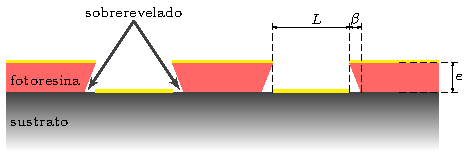
\includegraphics[width=\textwidth]{Esquemas/altura-ancho.pdf}
 				\end{subfigure}
 				\begin{subfigure}[t]{0.65\textwidth}
 				\includegraphics[width=\textwidth]{Imagenes/fotoresina_perfil.jpg}
 				\end{subfigure}
 				\caption[Perfil de fotorresina\index{fotorresina} para el decapado\index{decapar} o\textit{ lift-off}]{Arriba: esquema de la fotoresina depositada y revelada, donde se muestra la relación de espesor\index{espesor} respecto del ancho de línea y el sobrerevelado\index{sobrerevelado} necesario para un correcto decapado\index{decapar}. Abajo: corte por FIB\index{FIB} para evaluar el sobrerevelado\index{sobrerevelado} y espesor\index{espesor} obtenido luego de la transferencia por litografía.}
 				\label{fig:undercut}
 				\end{figure}

 	   		 La variable más delicada, es, sin lugar a dudas, el tiempo de revelado, ya que es la que compensa los errores acumulados en el proceso. Cualquier irregularidad en el sistema de iluminación, inhomogeneidades en el espesor\index{espesor} o calentamiento desparejo se ve reflejado en tiempos de revelado\index{revelado} diferenciales para diferentes sectores. Dicho esto, mientras más extenso el sustrato, más difícil es lograr un revelado\index{revelado} parejo. Es, también en este paso, donde se regula el <<sobrerevelado>> o, del inglés \textit{undercutting}\index{undercutting@\textit{undercutting}}, perfil necesario para que no se deposite metal en los laterales de la fotorresina\index{fotorresina} (figura \ref{fig:undercut}). El parámetro $\beta$ es la medida del sobrerevelado\index{sobrerevelado}, que es la diferencia entre la proyección en el sustrato\index{sustrato} de la superficie\index{superficie} superior y la superficie\index{superficie} inferior de la resina. Un $\beta\!\!\approx$\SI{500}{\nm} es el ideal para obtener buenos resultados en el procesos de \textit{lift-off}\index{lift@\textit{lift-off}}. 
 
 	         En la secuencia de imágenes de microscopia óptica de la figura \ref{fig:revelado} se muestra cómo evoluciona el revelado\index{revelado} con el tiempo y, en particular, se ve en la última imagen de esta secuencia, el resultado final de la etapa de litografía\index{litografía} y como el diseño resultó transferido de manera precisa.

 				%Imagnes revelado
 				\begin{figure}[th!]
			 	   	    \centering
			 	   	    \begin{subfigure}[t]{0.495\textwidth}
			        	\includegraphics[width=\textwidth]{Imagenes/revelado1.jpg}
			       		\end{subfigure}
			     		\begin{subfigure}[t]{0.495\textwidth}
			     		\includegraphics[width=\textwidth]{Imagenes/revelado2.jpg}
			    		\end{subfigure}
			     		\begin{subfigure}[t]{0.495\textwidth}
						\vspace*{-0.3cm}
			     		\includegraphics[width=\textwidth]{Imagenes/revelado3.jpg}
			        	\end{subfigure}
						\begin{subfigure}[t]{0.495\textwidth}
			     		\vspace*{-0.3cm}
			     		\includegraphics[width=\textwidth]{Imagenes/revelado4.jpg}
			        	\end{subfigure}
			     		\caption[Revelado en función del tiempo]{Tiempos crecientes de revelado: \SI{2.5}{min},\SI{3.5}{min},\SI{4.5}{min} y \SI{6}{min}). Se aprecia como se disuelve la resina en la solución reveladora indicado por el cambio de color a medida que disminuye el espesor\index{espesor}. Se muestra en la última microscopía\index{microscopía} el reveladio completo con un 20\% de tiempo adicional para crear el perfil negativo de las paredes, necesario para el proceso de\textit{ lift-off}.}
			     		\label{fig:revelado}\index{lift@\textit{lift-off}}
			     	   	\end{figure}

 		      Se llevó a cabo una segunda etapa de litografía\index{litografía} (luego del depósito\index{depósito} de Ti\index{titanio}\textbar Au\index{oro} para los electrodos) para colocar una resina fotocurable, epoxi\index{epoxi}, de alta viscosidad que genera estructuras de hasta \SI{100}{\um} de altura. En la fotografía de la figura \ref{fig:su8} se destaca la alta viscosidad de la misma al momento de hacer el deposito por \textit{spincoating}. Nuevamente los datos para trabajarla se obtuvieron de la hoja de datos del fabricante\cite{Su8,Microchemicals2014} y los detalles experimentales fueron expuestos en  sección \ref{sec:fotolito}, pág. \pageref{sec:fotolito}. Esta resina se usó para hacer la celda electroquímica\index{electroquimico}, la cual puede contener un volumen aproximado \SI{2}{\ul} de solución. En las microscopias de la figura \ref{fig:resultados-su8} se muestra el resultado obtenido luego de alinear y depositar esta resina expoxi\index{resina!expoxi}\index{epoxi}.

 				%Figura SU8 + alineacion + microscopia die con Su8
 				%Figura esquema undercutting
 				\begin{figure}[h!]
 				\centering
 				\includegraphics[width=\textwidth]{Imagenes/SU8.jpg}
 				\caption[Depósito de la resina expoxi\index{resina!expoxi}\index{epoxi} SU8]{Depósito por \textit{spin-coating }de la resina expoxi para encapsular. Se destaca la alta viscosidad de la misma, lo que permite formar paredes de hasta \SI{100}{\um} de espesor\index{espesor}.}
 				\label{fig:su8}\index{spin@\textit{spin-coating}}
 				\end{figure}

 				%Figura esquema undercutting
 				\begin{figure}[bh!]
			 	   	    \centering
			 	   	    \begin{subfigure}[t]{0.495\textwidth}
			        	\includegraphics[width=\textwidth]{Imagenes/alineacionSU8.pdf}
			       		\caption{Alineación de la segunda máscara\index{máscara} con la pelicula de Ti\index{titanio}\textbar Au\index{oro} ya depositada.}
			         	\label{fig:alineacion}
			     		\end{subfigure}
			     		\begin{subfigure}[t]{0.495\textwidth}
			     		\includegraphics[width=\textwidth]{Imagenes/DIE-SU8.pdf}
			    		\caption{Microscopía de uno de los sensores\index{sensor} con la celda integrada.}
			     		\label{fig:die-su8}	
						\end{subfigure}
						\caption[Alineación y celda integrada en SU8]{Resultados de la alineación de la capa de los electrodos con la máscara\index{máscara} para transferir la fotoresina expoxi\index{resina!expoxi}\index{epoxi} (a) y, (b) detalle de un sensor\index{sensor} terminado con celda EQ.}
			     		\label{fig:resultados-su8}
			     	   	\end{figure}

 		\subsection{Películas delgadas de Au}

		 Como ya se mencionó anteriormente, los electrodos de los sensores\index{sensor} son de Au\index{oro} y fueron depositados por la técnica de pulverización catódica\index{pulverización catódica} o mas comúnmente conocida por su nombre en inglés \textit{sputtering}\index{sputtering@\textit{sputtering}}. La fabricación consistió primero en depositar una capa de al menos de \SI{20}{\nm} de espesor\index{espesor}, llamada capa de  adherencia, la misma puede ser indistintamente de Ti\index{titanio} o Cr\index{cromo}, la cual promueve la adherencia\index{adherencia} del Au; sin esta capa el Au\index{oro} no adhiere sobre superficie\index{superficie}s no metálicas.\cite{Hieber1976} Una vez depositada la capa adherente y sin romper el vacío de la cámara del equipo, se depositaron \SI{150}{nm} de Au. El espesor\index{espesor} resultó ser el óptimo para lograr un electrodo mecánicamente robusto y con buenas propiedades de conducción eléctrica pero suficientemente delgado para que las películas delgadas mesoporosas sean continuas entre los electrodos y el sustrato. Para cada caso, en condiciones constantes, se puede realizar una curva de calibración. La misma se consigue graficando el espesor\index{espesor} de las películas depositadas en función del tiempo, con el objetivo de establecer la tasa de depósito\index{depósito} y así poder controlar el espesor\index{espesor} de la película. 

		 Se optimizaron las condiciones de \textit{sputtering}\index{sputtering@\textit{sputtering}} para obtener películas homogéneas tanto en espesor\index{espesor} como superficialmente. Para lograrlo se variaron los parámetros relevantes de la técnica, que son: la aceleración de los iones, determinada por diferencia de tensión entre el cátodo\index{cátodo} y ánodo\index{anodo @ ánodo}; la densidad de corriente y el flujo de Ar\index{argón}. Una vez establecidas dichas condiciones se mantuvieron constante a lo largo de la tesis. El espesor\index{espesor} de las películas metálicas, $d$, se reguló controlando el tiempo de depósito, $t$. De acuerdo a los los trabajos de Sigmund\index{Sigmund}\cite{sigmund1968} y Seah\index{Seah}\cite{Seah2005} éstas variables son directamente proporcionales según la ecuación \ref{eq:sputt}, donde $J$ es la densidad de corriente, $Y$ el rendimiento de la pulverización, $r$ el radio átomico del material y $e_o$ la carga del electrón\index{electrón}.

	 			\begin{equation}
	 				d=\left(\frac{JYr^3}{e_o}\right)t
	 				\label{eq:sputt}
	 			\end{equation}

		 Las condiciones de depósito\index{depósito} de cada una de las sucesivas capas se detallan en la tabla \ref{tabla:sputt1}, pág. \pageref{tabla:sputt1}, para las películas metálicas y en la tabla  \ref{tabla:sputt2}, pág. \pageref{tabla:sputt2} para el SiO$_2$. 


		 Para establecer las tasas de depósitos de uno de los materiales pulverizados, se midió el espesor\index{espesor} resultante de las películas por diferentes técnicas. Para monocapa\index{monocapa}s de Au\index{oro} y espesor\index{espesor}es pequeños típicamente menores a los \SI{30}{\nm}, se utilizó elipsometría espectrométrica, los detalles experimentales y la base de la técnica ya fueron discutidos en la sección \ref{sec:elipso}, pág. \pageref{sec:elipso}. Para evaluar el apilamiento de sucesivas capas, inspeccionar la homogeneidad tanto en espesor\index{espesor} como superficial, se utilizó microscopía\index{microscopía} electrón\index{electrón}ica de barrido (MEB) y haz focalizado de iones (FIB), técnica que permite hacer cortes e inspecciones de secciones transversales de los depósitos en distintos puntos. 
		
		 En la figura \ref{fig:FIB_electrodos} se puede ver un corte transversal de los electrodos, realizado por FIB\index{FIB}, donde se ven los espesor\index{espesor}es de ambas películas metálicas (Ti, capa adherente y Au), así como la capa dieléctrica de SiO$_2$. También se aprecia la buena homogeneidad en el espesor\index{espesor} de cada una de las capas y en la superficie\index{superficie} de la capa de Au, donde ocurrirá finalmente el intercambio electrón\index{electrón}ico entre las especies redox. Midiendo los espesor\index{espesor}es de las capas depositadas a distintos tiempos, podemos establecer la tasa de deposito, obtenida de la pendiente del figura \ref{fig:calibracionAu}. Como ya se mencionó en reiteradas ocasiones, es de suma importancia conocer y controlar los espesor\index{espesor}es de cada una de las capas, ya sean películas delgadas mesoporosas, densas o metálicas.


		 		%figura FIB\index{FIB} de los electrodos
						  \begin{figure}[h!]
						  \begin{center}
						  \includegraphics[width=0.80\textwidth]{Imagenes/Perfil.jpg}
						  \caption[Sección trasversal de los eletrodos]{Corte transversal de los electrodos, donde se observan detalles de la bicapa Cr\index{cromo}\textbar Au\index{oro} depositada sobre una oblea\index{oblea} de silicio\index{silicio} con un depósito\index{depósito} aislante de SiO$_2$.}
						  \label{fig:FIB_electrodos}
						  \end{center}
						  \end{figure} 	

				%Grafico de la curva de calibración para el Au
					   		\begin{figure}[h!]
					   		\begin{center}
							\includegraphics[width=0.75\textwidth]{Graficos/Espesor_Au.pdf}
							\caption[Curva de calibración para el espesor\index{espesor} de los electrodos]{Curva de calibración para establecer la tasa de de depósito\index{depósito} de la capa de Au. La misma se realizó por pulverización catódica\index{pulverización catódica} en las condiciones experimentales detalladas en la tabla \ref{tabla:sputt1}.}
							\label{fig:calibracionAu}
							\end{center}
							\end{figure}		  
		
  		\subsection{Decapado de la fotorresina\index{fotorresina} o\textit{ lift-off}}

		 %En algun lugar se puede decir que se elijio lift-off en lugar de etching porque es mejor porque no se coloca fottoresina sobre los electrodos, etc, etc.

		 La última etapa de la fabricación de los electrodos es el decapado\index{decapar} de la fotorresina\index{fotorresina}, técnica que se conoce mas comúnmente con el nombre en inglés, \textit{lift-off}\index{lift@\textit{lift-off}}. Consiste en disolver la fotorresina\index{fotorresina} que queda luego del revelado\index{revelado} y que se utilizó a modo de capa de sacrificio. En la figura \ref{fig:undercut} se pueden ver los sitios por donde da comienzo la disolución. La fotoresina utilizada es completamente soluble en acetona. Cabe destacar, nuevamente, que es importante la disontinuidad de la película de oro\index{oro} para que tenga éxito esta etapa, ya que, si existe continuidad entre la parte que se quiere dejar y la que no, se generan imperfecciones en los bordes, o se desprende el metal de partes que no se desea. Para ello es muy importante saber bien los espesor\index{espesor}es que se logran durante el depósito, tanto de fotorresina\index{fotorresina} como de película de Au, para regular la distancia que quede entre el metal en el sustrato\index{sustrato} y el metal sobre la resina. El esquema y la microscopía\index{microscopía} de la figura\ref{fig:undercut} presentado anteriormente en la pág. \pageref{fig:undercut} ejemplifica bien esta situación.

					  %Oblea Terminada V1
					  \begin{figure}[ht!]
					  \begin{center}
					  \includegraphics[width=\textwidth]{Imagenes/lift-off.jpg}
					  \caption[Proceso de decapado\index{decapar} o\textit{ lift-off}]{Proceso de decapado\index{decapar} o\textit{ lift-off}. Fotografía correpondiente a los electrodos del primer diseño, donde se muestra como a medida que se disuelve la fotorresina\index{fotorresina} se va levantando el metal que está sobre ella.}
					  \label{fig:ultrasonido}\index{lift@\textit{lift-off}}
					  \end{center}
					  \end{figure}

		 Por último, es importarte saber que es necesario aplicar ultrasonido. No alcanza con una simple inmersión de la oblea\index{oblea} en solvente sino que se precisa mantener una constante convección para la completa remoción de la fotorresina\index{fotorresina}. A su vez, este proceso de constante movimiento evita el redepósito del metal liberado sobre los electrodos (figura \ref{fig:ultrasonido}), ya que si ocurre este fenómeno es muy difícil, una vez que se seca la oblea, remover el metal de desperdicio que se adhiere a los electrodos. Es en esta etapa final del proceso donde se demuestra si resultaron efectivas las etapas de limpieza y revelado. De haber algún residuo remanente durante la limpieza del sustrato\index{sustrato} o haber efectuado un revelado\index{revelado} incompleto, se producirá indefectiblemente el desprendimiento de los electrodos del sustrato.

		 Finalmente, en las figuras \ref{fig:ObleaV1} y \ref{fig:ObleaV2}, se muestra el resultado final de la fabricación de los electrodos realizados en obleas de cuatro pulgadas (\SI{10}{\cm} de diámetro) para los dos diseños elaborados.

		 			  \clearpage
					  %Oblea Terminada V1
					  \begin{figure}[ht!]
					  \begin{center}
					  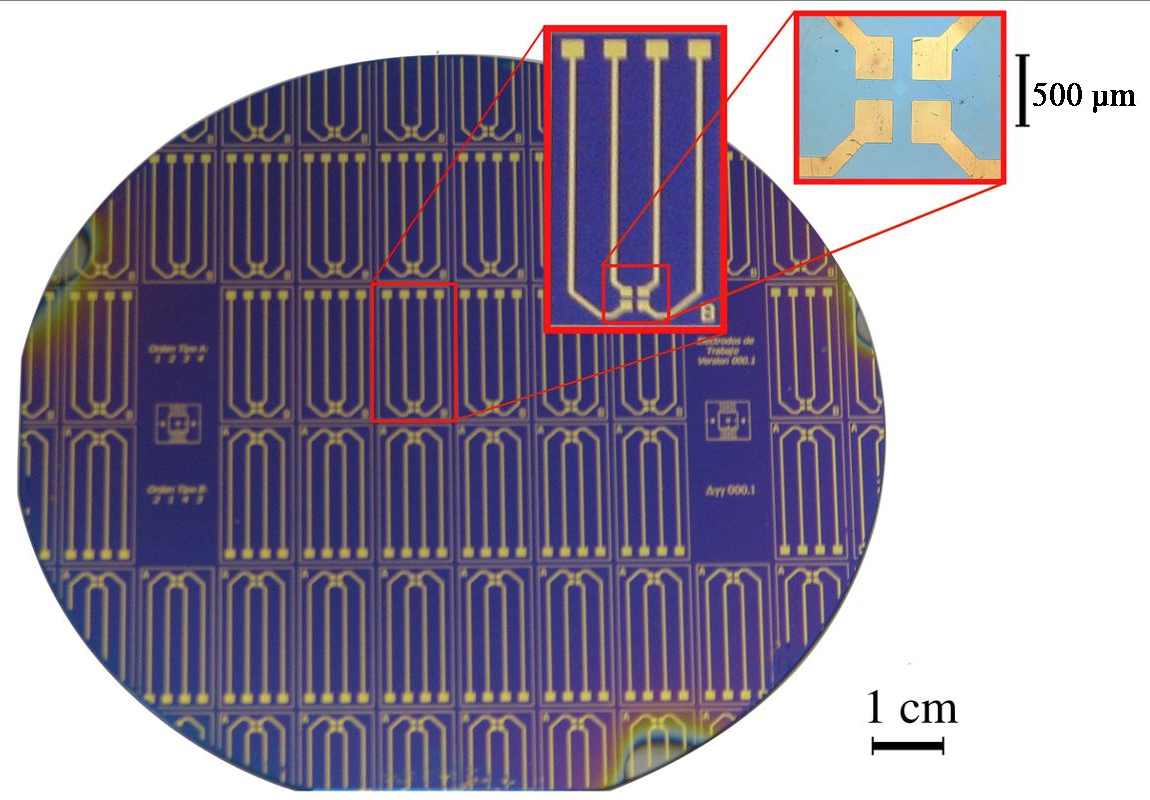
\includegraphics[width=0.90\textwidth]{Imagenes/ObleaV1.jpg}
					  \caption[Electrodos, primera versión]{Primer diseño de los sensores. Oblea de silicio\index{silicio} de \SI{10}{cm} de diámetro, capa de SiO$_2$ y 32 sensores\index{sensor} con cuatro electrodos de trabajo\index{electrodo!de trabajo} cada uno.}
					  \label{fig:ObleaV1}
					  \end{center}
					  \end{figure} 	

					  %Oblea Terminada V2
					  \begin{figure}[h!]
					  \begin{center}
					  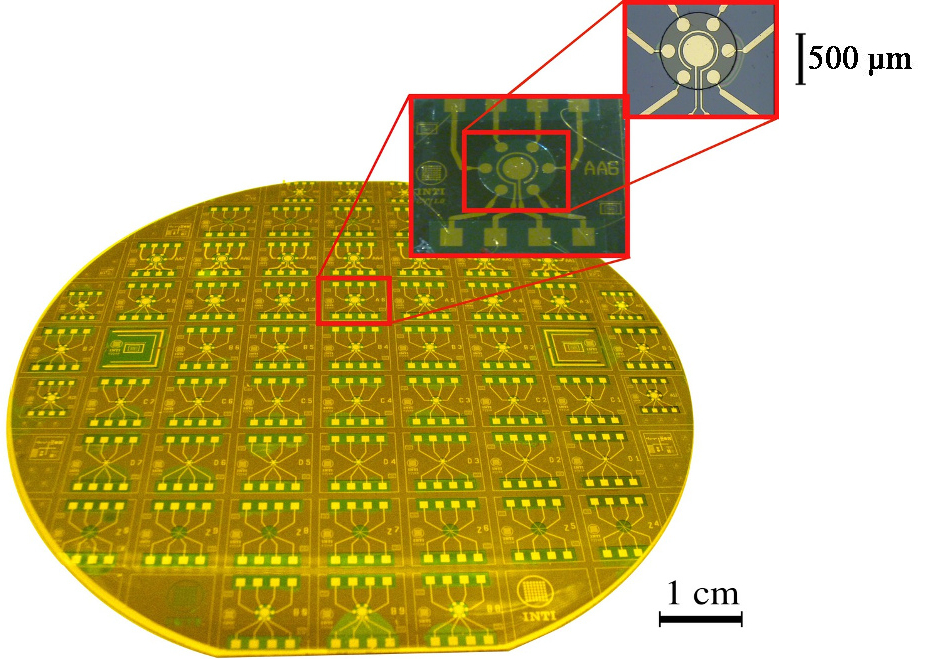
\includegraphics[width=0.90\textwidth]{Imagenes/ObleaV2.jpg}
					  \caption[Electrodos, segunda versión]{Segundo diseño de los sensores. Oblea de silicio\index{silicio} de \SI{10}{cm} de diámetro con 46 sensores\index{sensor} con 6 electrodos de trabajo\index{electrodo!de trabajo}, contraelectrodo\index{electrodo!contraelectrodo} y pseudoreferencia\index{pseudoreferencia}. También se muestra la celda electroquímica\index{electroquimico} depositada con resina expoxi\index{resina!expoxi}\index{epoxi} SU-8.}
					  \label{fig:ObleaV2}
					  \end{center}
					  \end{figure} 	
	
		\section{Caracterización de los electrodos}

		 Se dará cuenta en esta sección de las diferentes caracterizaciones y ensayos practicados sobre los electrodos de Au\index{electrodo!de Au}. Fundamentalmente la respuesta electroquímica\index{electroquimico}, ya que la base de los sensores\index{sensor} son las reacciones de óxido reducción. Es por ello que es necesario obtener electrodos de respuesta reproducible, confiable y fabricados por un proceso repetible y escalable. 

	\subsection{Respuesta electroquímica\index{electroquimico}}\label{sec:respuesta_sondas_au}
			 		
			Una vez que los resultados de la fabricación de los sensores\index{sensor} fueron óptimos se evaluó el desempeño electroquímico\index{electroquimico} de los mismos. En el capítulo \ref{chap:Materiales} se describe con detalle el montaje experimental para realizar las mediciones de voltametrías cíclica (VC). Se usaron como sonda\index{sonda}s electroquímica\index{electroquimico}s\index{electroquimico} ferro y ferricianuro de potasio\index{ferricianuro de potasio} (\Ferro\space y \Ferri, \fe), cloruro de hexaaminorutenio(III) (\aminorutenioCompleto, \ru) y ferroceno metanol\index{ferroceno metanol} (\ferroceno, \fc). La elección de estas sonda\index{sonda}s modelo tiene que ver fundamentalmente con la carga neta de cada una de ellas, y con la reversibildiad de los pares redox. Analizaremos ahora como fue la respuesta de los electrodos compuestos por películas delgadas de Au\index{oro} para cada una de estas sonda\index{sonda}s.
				
		\subsubsection*{Respuesta de ferro/ferricianuro de potasio}	 
			 	
		   En electroquímica\index{electroquimico} éste par rédox es frecuentemente utilizado para evaluar la calidad de electrodos. Esto se debe a que se trata de par rédox cuyas especies oxidada y reducida son moléculas económicas, fácil de conseguir, solubles en solución acuosa y se compartan de forma cuasireversible frente al intercambio electrón\index{electrón}ico electrodo-especie. La reacción que tiene lugar es la siguiente:
			 \begin{equation}
			 \schemestart 
			 Fe(CN)$_6^{4-}$  
			 \arrow{<=>[\scriptsize oxidación][\scriptsize reducción]}[0,1.5] 
			 Fe(CN)$_6^{3-}+e^-$ \schemestop
			 \end{equation}
		   Se espera, en la aproximación más simple, que sigan el comportamiento descrito por Randles-Sevcik\index{Randles-Sevcik}, donde la intensidad de pico ($i_p$) es proporcional a la concentración ($C$) y a la raiz cuadrada de la velocidad de barrido\index{velocidad!de barrido} $v$ según:
		  
		 	\begin{equation}
			i_p=0.4463nFAC\left(\frac{nFvD}{RT}\right)^{1/2}
			\label{eq:rs2}
			\end{equation}

			\begin{figure}[ht]
	 	    	\begin{subfigure}[t]{0.5\textwidth}
	         	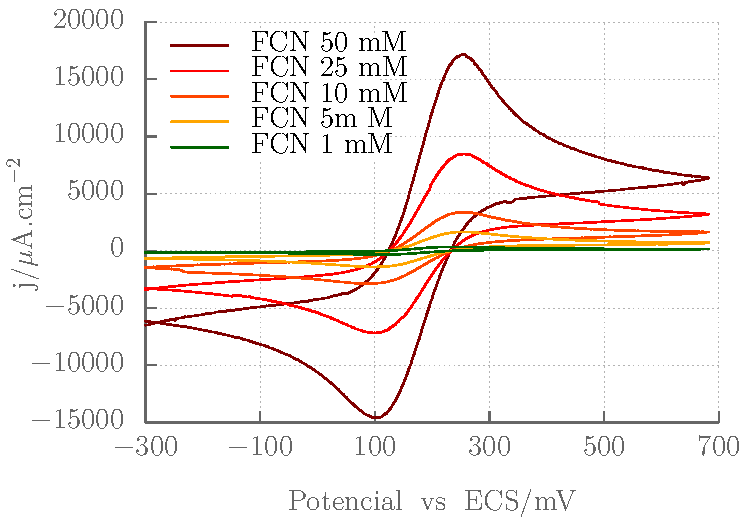
\includegraphics[width=\textwidth]{Graficos/Concentraciones_Fe.pdf}
	        	\caption{Voltametrías cíclicas para la cupla \fe\space a diferentes concentraciones. Todas medidas fueron tomadas a \SI{50}{\milli\volt\per\second}.}
	         	\label{fig:Fe_a}
	     		\end{subfigure}
     		 \begin{subfigure}[t]{0.495\textwidth}
	        	\includegraphics[width=\textwidth]{Graficos/Calibracion_Fe.pdf}
	       		\caption{Curva de calibración para distintas concentraciones de la cupla \fe. Valores tomados de la figura \ref{fig:Fe_a}.}
	         	\label{fig:Fe_b}
	     		\end{subfigure}
	     		%\vspace*{0.5cm}

 	     	\begin{subfigure}[t]{0.495\textwidth}
         		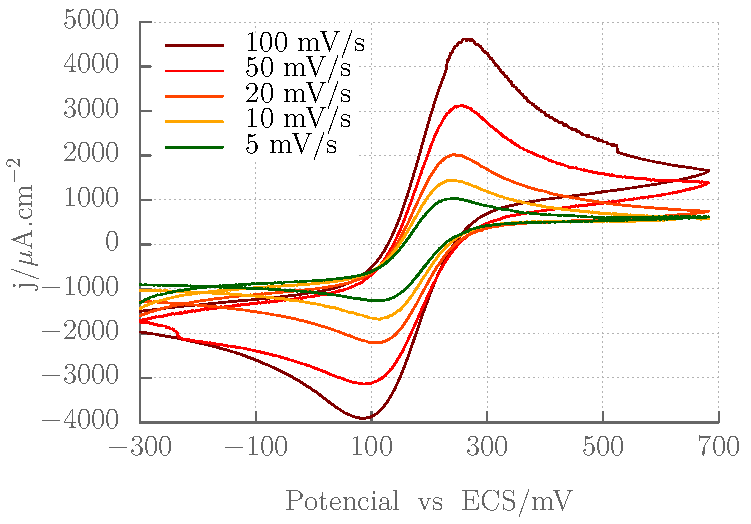
\includegraphics[width=\textwidth]{Graficos/Velocidades_Fe.pdf}
        	    \caption{Voltametrías cíclicas de una solución \SI{10}{\milli\Molar} de la cupla equimolar \fe\space para diferentes velocidades de barrido.}
        	    \label{fig:Fe_c}
     		 	\end{subfigure}
     	 	\begin{subfigure}[t]{0.495\textwidth}
        		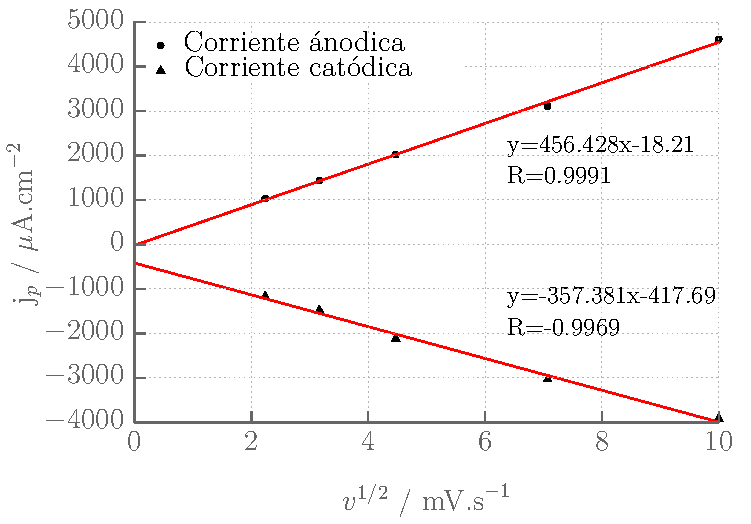
\includegraphics[width=\textwidth]{Graficos/VelocidadesCal_Fe.pdf}
       			\caption[Respuesta a diferentes velocidades de barrido para \fe]{Dependencia de la corriente de pcio con la velocidad de barrido\index{velocidad!de barrido} para \fe\space \SI{10}{\milli\Molar}. Valores extraidos de la figura \ref{fig:Fe_c}.}
         		\label{fig:Fe_d}
     			\end{subfigure}
     		 \caption[Respuesta electroquímica\index{electroquimico} para \fe]{(a) Respuesta electroquímica\index{electroquimico} de la cupla equimolar \fe\space para distintas concentraciones, (b) curva de calibración para dichas concentraciones. (c) Densidad de corriente en función con la velocidad de barrido\index{velocidad!de barrido}, (d) dependencia de la densidad de corriente de pico con la raíz cuadrada de la velocidad de barrido\index{velocidad!de barrido}. Todos los voltagramas fueron tomadas con contraelectrodo\index{electrodo!contraelectrodo} de Pt\index{platino}, en 0,1M de NaCl como electrolito soporte y utilizando como referencia ESC.}
     		 \label{fig:ferro-ferri-CV}
     		 \end{figure}

     		 Con el propósito de corroborar este comportamientos, se realizaron experimentos de VC a diferentes concentraciones de la sonda\index{sonda} (figuras \ref{fig:Fe_a} y  \ref{fig:Fe_b}) y a distintas velocidades de barrido (figuras \ref{fig:Fe_c} y  \ref{fig:Fe_d}). Resultaron de especial utilidad la curva de calibración y la respuesta frente a distintas velocidades de barrido. Para cualquiera de estás velocidades los voltagramas conservan constantes los valores de $E^\circ$, indicativo de una buena trasferencia de carga entre el electrodo y la sonda\index{sonda}. Además se destaca la relación lineal de j$_p$ con $v^{1/2}$ verificando la ecuación de Randles-Sevcik\index{Randles-Sevcik} (ec. \ref{eq:rs2}).		  	  
  					
		  	 Con los resultados obtenidos para estas voltametrías se puede sugerir que el sistema responde a un proceso de difusión\index{difusión} lineal en un plano semiinfinito, lo cual era lo que se esperaba en primer orden para un sistema en el que el electrodo esta embebido en solución con el analito electroactivo en solución de electrolito soporte {(\SI{0,1}{\milli\Molar} KCl, pH\index{pH}=$5.5$)\cite{Wi2000,Pumera2007,Gewirth2004,Villullas2000}.

	 	\subsubsection*{Respuesta del cloruro de hexaaminorutenio(III)}
	
	 	 El cloruro de hexaaminorutenio(III) se utilizó extensivamente en este trabajo, gran parte de la discusión del capítulo \ref{chap:Electroquimica} tiene por eje la adsorción\index{adsorción} de este complejo en las películas delgadas mesoporosas. Esta molécula\index{moléculas} en solución se disocia para formar el complejo \aminorutenio. La reacción rédox que tiene lugar es la siguiente:
	 		 	 	  		\begin{equation}
	 		 	 	 			\schemestart 
					 			 Ru(NH\index{amoniaco}$_3$)$_6^{2+}$  
					 			 \arrow{<=>[\scriptsize oxidación][\scriptsize reducción]}[0,1.5] 
					 		 	 Ru(NH\index{amoniaco}$_3$)$_6^{3+}+e^-$ \schemestop 
	 		 	 	 		\end{equation}
	 	  El intercambio entre los estados de oxidación Ru$^{3+}$/Ru$^{2+}$, responde a un proceso electroquímico\index{electroquimico} reversible, en el cual podemos fácilmente reducir u oxidar el complejo variando el potencial del electrodo de trabajo\index{electrodo!de trabajo}. Habiendo ya comprobado, con el \fe, el buen desempeño de los electrodos respecto de la velocidad de barrido\index{velocidad!de barrido}, se eligió un valor \SI{50}{\milli\volt\per\second} para las voltametrías cíclicas (de uso frecuente para este tipo de mediciones). Se llevaron a cabo una serie de VC para varias concentraciones de la sonda\index{sonda}, con el objetivo de elaborar la correspondiente curva de calibración para \aminorutenio. Se verifica de estos voltagramas el buen desempeño EQ de los electrodos referente a la transferencia de electrones.
		
			 \begin{figure}[ht]
	 	     \begin{subfigure}[t]{0.495\textwidth}
	         	\includegraphics[width=\textwidth]{Graficos/Concentraciones_Ru.pdf}
	        	\caption{Voltametrías cíclicas para \ru\space a diferentes concentraciones.}
	         	\label{fig:Ru_a}
	     		\end{subfigure}
     		 \begin{subfigure}[t]{0.495\textwidth}
	        	\includegraphics[width=\textwidth]{Graficos/Calibracion_Ru.pdf}
	       		\caption{Curva de calibración para la especie \ru. Los valores fueron tomados de la figura \ref{fig:Ru_a}.}
	         	\label{fig:Ru_b}
	     		\end{subfigure}
	     		\label{rutenio}
	     		\caption[Respuesta electroquímica\index{electroquimico} para \ru]{(a) Voltametrías cíclicas para soluciones de \ru\space de distinta concentración y, (b) curva de calibración para dichas concentraciones. Todos los voltagramas fueron tomados a \SI{50}{\milli\volt\per\second} con contraelectrodo\index{electrodo!contraelectrodo} de Pt\index{platino} en una solución \SI{0.1}{\milli\Molar} de NaCl y utilizando de referencia ESC.}
	     	 \end{figure}
			 		 	 
		\subsubsection*{Respuesta del ferroceno metanol}
 	 	 
 	 	  A diferencia de las sonda\index{sonda}s anteriores la especie reducida del \fc\space tiene carga neta, por lo que se puede esperar que no tenga interacciones de tipo electrostáticas con las películas delgadas mesopoporosas. Por lo que es de  Es por ello que resultó imprescindible para sacar conclusiones acerca de los fenómenos de transporte\index{transporte} y comparar sistemas calcinados con sistemas no clacinados, como ya se discutió ampliamente en el capítulo anterior. 
 	 	  La reacción de oxidación/reducción para esta molécula\index{moléculas} es la siguiente:
 	 	 			%Ecuación redox para el Ferroceno
 	 				 \begin{equation}
 	 	 				\begin{aligned}
 	 	 				\includegraphics[scale=0.75]{Esquemas/Redox-Fc.pdf}
 	 	 				\end{aligned}
 	 	 			 \end{equation}
 	 	  
 	 	 De la misma forma que se realizó para las otras sonda\index{sonda}s, se confeccionó una curva de calibración para distintas concentraciones de \fc\space, la figura \ref{Fig:Fc} muestra la respuesta electroquímica\index{electroquimico} correspondiente sobre electrodos de Au\index{electrodo!de Au}.
 	 				
 	 				%Graficos para el Ferroceno
		 		 \begin{figure}[ht]
		 	      \begin{subfigure}[t]{0.495\textwidth}
		          	\includegraphics[width=\textwidth]{Graficos/Concentraciones_Fc.pdf}
		         	\caption{Voltametrías cíclicas para \fc\space a diferentes concentraciones, \SI{1}{\milli\Molar}, \SI{5}{\milli\Molar} y \SI{10}{\milli\Molar}.}
		          	\label{fig:Fc_a}
		      		\end{subfigure}
		      	 \begin{subfigure}[t]{0.495\textwidth}
		          	\includegraphics[width=\textwidth]{Graficos/Calibracion_Fc.pdf}
		         	\caption{Curva de calibración para la especie \fc. Los valores fueron tomados de la figura \ref{fig:Fc_a}.}
		          	\label{fig:Fc_b}
		      		\end{subfigure}
		      	 \caption[Respuesta electroquímica\index{electroquimico} para \fc]{(a) Voltametrías cíclicas para soluciones de \fc\space de distinta concentración y, (b) curva de calibración para dichas concentraciones. Todos los voltagramas fueron tomadas a \SI{50}{\milli\volt\per\second} con contraelectrodo\index{electrodo!contraelectrodo} de Pt\index{platino} en una solución \SI{0.1}{\Molar} de NaCl y utilizando ESC como referencia.}
		      	 \label{Fig:Fc}
	      		 \end{figure}

		 En la tabla \ref{tabla:sondas} se resumen las características y los resultados de las voltametrías cíclicas para cada una de las sonda\index{sonda}s modelo elegidas. Las variables calculadas fueron la diferencia de potenciales entre el pico de corriente anódico y catódico, de forma de evaluar la reversibilidad de la reacción y capacidad de transferencia electrón\index{electrón}ica de los electrodos y el coeficiente de difusión\index{difusión} de una especie libre en un electrodo plano semiinfinito. Durante todo el desarrollo de la tesis se utilizaron estos resultados con ánimos de comparar los voltagramas sobre los electrodos desnudos y sobre los electrodos con la película mesoporosa.
		  
		  %Tabla resultados EQ
		     \begin{table}[ht]
		     \vspace*{0.5cm}
	  		  \caption[Sondas electroquímica\index{electroquimico}s\index{electroquimico}]{Características de las sonda\index{sonda}s electroactivas utilizadas a lo largo de la tesis. Cálculo del coeficiente de difusión\index{difusión} ($D$) para difusión\index{difusión} en un plano simiinfinito a \SI{25}{\celsius}.}
	  		  \begin{tabular}{>{\raggedright\arraybackslash}m{2.2cm}>{\centering\arraybackslash}m{2.3cm}>{\centering\arraybackslash}m{2.3cm}>{\centering\arraybackslash}m{1.5cm}>{\centering\arraybackslash}m{1.72cm}}
	  		  \toprule
			  \multirow{2}{*}{Sonda}  	& Carga especie  & Carga especie  & \multirow{2}{*}{$\Delta$E(mV)} & \multirow{2}{*}{$D$(cm$^2$s$^{-1}$)} \\
			     		    & \hspace*{-0.79cm}reducida      & \hspace*{-0.85cm}oxidada  &	   & \\ \midrule
	    	  \ferroferri	& \multirow{1}{*}{$4-$}  		& $3-$	     			   &  150  &  \num{2.0e-7}\\ \midrule
	  		  \aminorutenio & $2+$							& $3+$					   &  80   &  \num{5.5e-6} \\ \midrule
	  		  \raisebox{-.5\height}{\includegraphics[scale=0.5]{Esquemas/Fc.pdf}}   &  \hspace*{-0.29cm}0 & 1+ &  103 & \num{1.9e-6} \ \\   		 
	  		  \bottomrule
	    	  \end{tabular}
	   		  \label{tabla:sondas}
			  \end{table}
		
			\pagebreak			

    \subsection{Incompatibilidad \textit{top-down/bottom-up}}

  			Una vez demostrado el óptimo desempeño electroquímico\index{electroquimico} de los microelectrodo\index{electrodo!microelectrodo}s fabricados por técnicas \textit{top-down}\index{top-down@\textit{top-down}}, la siguiente etapa consintió en el depósito\index{depósito} de la película mesoporosa\index{película!mesoporosa} sobre los electrodos. Ya se discutió a lo largo del capítulo \ref{chap:Mesoporosos} las técnicas de depósito, el control sobre la síntesis, los parámetro para obtener películas de diferente porosidad, espesor\index{espesor}, adherencia, etc.

  			Previo a los resultados discutidos y analizados en el capítulo \ref{chap:Mesoporosos} y basándose en trabajos similares\cite{Otal2006,Calvo2009,Fattakhova-Rohlfing2007,Rohlfing2005}, donde utilizan mediciones electroquímica\index{electroquimico}s\index{electroquimico} como herramienta para establecer propiedades de las \pdm, se realizaron experimentos preliminares y equivalente para evaluar el transporte\index{transporte} en películas delgadas mesoporosas de SiO$_2$. En los trabajos citados utilizan vidrio\index{vidrio} ITO o vidrio\index{vidrio} FTO como electrodos y llevan a cabo mediciones electroquímica\index{electroquimico}s\index{electroquimico} sobre sistemas clásicos, películas calcinadas y electrodos no miniaturizados. En este trabajo las primeras medidas se realizaron sobre películas mesoporosas de SiO$_2$ estructuras con F127, depositadas sobre películas delgadas de Au\index{oro} y condensadas y extraídas por la vía de calcinaciones (\SI{350}{\celsius}). Los resultados preliminares de estas mediciones (previos al desarrollo de la discusión sobre transporte\index{transporte} del capítulo \ref{chap:Electroquimica}) no fueron los esperados. Mostraban, o voltagramas <<planos>>, o curvas donde la respuesta no era óptima, propia de electrodos con alta resistencia o limitados en la cinética de transferencia electrón\index{electrón}ica.

  			El estudio de porqué en estos sistemas calcinados la respuesta era muy diferente a la reportada, se encaró de forma sistemática. Se plantearon tres hipótesis: 1) contaminación de los reactivos, 2) poros bloqueados, 3) difusión\index{difusión} de impurezas producto de la calcinación\index{calcinación}.

  			Para evaluar la hipótesis contaminación en los reactivos, se repitió la preparación de los soles, de las sonda\index{sonda}s, se reemplazaron los solventes y el electrolito soporte por nuevos. La respuesta electroquímica\index{electroquimico} seguía siendo deficiente por lo que se descartó esta hipótesis. 

  			Las hipótesis de poros bloqueados quedó descartada luego de realizar repetidas mediciones de eliposoporosimetría ambiental demostrando la buena accesibilidad\index{accesibilidad} y porosidad\index{porosidad} que mostraban las películas delgadas mesoporosa\index{película!mesoporosa} sometidas a  calcinación\index{calcinación} (ver sección \ref{sub:m_todo_de_calcinaci_n}, pág. \pageref{sub:m_todo_de_calcinaci_n} y figura \ref{fig:F127_epa_psd_cal}, pág. \pageref{fig:F127_epa_psd_cal}).

  			Para evaluar la hipótesis de contaminantes que difunden debido a la temperatura se hicieron experimentos con muestras control, las cuales consistieron en electrodos de Au\index{electrodo!de Au} sometidos a calcinación\index{calcinación} pero sin depositar el sol\index{sol} sobre ellos. En resumen se sometió los electrodos de Au\index{electrodo!de Au} desnudos a condiciones de humedad y temperatura idénticos a las utilizadas en el proceso de síntesis de las \pdm\space (ver el proceso descrito en la sección \ref{sec:cond_y_extr}, pág. \pageref{sec:cond_y_extr}). La respuesta electroquímica\index{electroquimico} seguía siendo defectuosa, por lo que se consolidó la hipótesis de difusión\index{difusión} de contaminantes por la temperatura utilizada (\SI{350}{\celsius}). 

  			Se llevaron a cabo una serie de caracterizaciones sobre las películas delgadas de Au\index{oro} sometidas a la calcinación\index{calcinación} para comprender como fueron afectadas e interpretar la respuesta electroquímica\index{electroquimico} cuando se las usó como electrodos.
		
		\subsubsection{Resistencia superficial}

			Se midió la resistencia superficial a de las películas delgadas de Au, con el objetivo de corroborar algún cambio respecto en las propiedades eléctricas de los electrodos luego de ser sometidos a las condiciones de procesos para la síntesis de las \pdm. El aumento de la resistividad puede traer emparejados deformaciones en los voltagramas, caída óhmica o separación de los potenciales de pico. Las mediciones se llevaron a cabo sobre tres muestras: una sin tratamiento térmico, otra calcinada a \SI{350}{\celsius} y una tercera llevada también a \SI{350}{\celsius} pero en atmósfera\index{atmósfera} de alto vacío\index{alto@alto vacío} (\SI{e-5}{\milli\bar}). Los resultados se resumen en la tabla \ref{tabla:resistencia}, donde se corrobora que la resistencia por cuadrado aumenta para las muestras sometidas a tratamiento térmico, posiblemente debido a la difusión\index{difusión} de impurezas hacia la superficie\index{superficie}. Dichas impurezas pueden provenir del Au, de la capa de adherencia\index{adherencia} o del sustrato\index{sustrato} (silicio o vidrio).

				\begin{table}[ht!]
			  		  \caption[Resistencia superficial de los electrodos]{Resistencia superficial de los electrodos con y sin tratamiento térmico.} 
			  		  \begin{tabular}{>{\raggedright\arraybackslash}m{4.2cm}>{\raggedright\arraybackslash}m{7.075cm}} 
			  		  \toprule
					  Muestra & Resistividad superficial $(\Omega/_{\square})$  \\ \midrule
			      	  Au\index{oro} \SI{350}{\celsius} 		  	& $3.720 \pm 0.001$		 \\	  
			      	  Au\index{oro} \SI{350}{\celsius} en vacío	& $3.685 \pm 0.001$		 \\	  
			      	  Au\index{oro} \SI{25}{\celsius}    	  		& $0.595 \pm 0.001$		 \\ 
			      	  \bottomrule
			    	  \end{tabular}
			    	  \label{tabla:resistencia}
			   		  \end{table}	
	
		\subsubsection{Análisis de la superficie\index{superficie} por XPS\index{XPS}}

			Se ha reportado trabajos donde demuestran que es posible la difusión\index{difusión} hasta la superficie\index{superficie} del electrodo, de metales provenientes de la capa de adherencia\index{adherencia} e incluso de iones provenientes del sustrato\index{sustrato} \cite{Alonso1990,Moody2003}. Para ello se decidió analizar la superficie\index{superficie} de los electrodos mediante espectroscopia de fotoelectrones emitidos por rayos X\index{rayos Xssh} (XPS). Se llevó a cabo un experimento en el cuál se depositaron dos electrodos de Cr\index{cromo}\textbar Au\index{oro} sobre silicio, uno de ellos fue sometido a tratamiento térmico mientras que el otro no. Los resultados se muestran en el gráfico de la figura \ref{fig:XPS}, donde se evidenció la difusión\index{difusión} hacia la superficie\index{superficie}, de cromo\index{cromo} ligado a oxígeno. Esto sugiere que el cromo, utilizado como capa de adherencia, se oxida y difunde cuando los sensores\index{sensor} son sometidos a una temperatura de \SI{350}{\celsius}.

				\begin{figure}[ht!]
		 	       	\begin{center}
		 	       	\includegraphics[width=0.85\textwidth]{Graficos/XPS.pdf}
		        	\caption[XPS de películas delgadas de Cr\index{cromo}\textbar Au]{Espectroscopia de fotoelectrones emitidos por rayos (XPS) correspondiente a películas delgadas de Cr\index{cromo}\textbar Au\index{oro} con y sin tratamiento térmico. Obsérvese los picos correspondiente al cromo\index{cromo} y el aumento de la intensidad relativa del pico correspondiente al oxígeno, sugiriendo la difusión\index{difusión} de Cr\index{cromo}$_x$O$_y$ hacia la superficie\index{superficie} de los electrodos.}
		         	\label{fig:XPS}
		         	\end{center}
		     		\end{figure}

		\subsubsection{Microscopía electrón\index{electrón}ica de barrido}
			  		
			 Una vez demostrado que es posible la difusión\index{difusión} de impurezas a \SI{350}{\celsius} se realizaron imágenes por microscopía\index{microscopía} de barrido electrón\index{electrón}ico para estudiar como afecta dicho tratamiento la morfología de las películas. En la figura \ref{fig:Au_compTT} se comparan depósitos de Cr\index{cromo}\textbar Au\index{oro} tratados térmicamente con depósitos no tratados. Se observa un crecimiento en el tamaño de partícula para los sometidos a tratamiento térmico, más específicamente a \SI{350}{\celsius}, temperatura usada para la vía clásica de síntesis de \pdm. Este hecho demuestra que esta temperatura es suficiente, para, al menos, producir un aumento en el tamaño de los cristales de las películas delgadas de oro. Dicha transformación también fue reportada a una temperatura menor, de \SI{300}{\celsius} por \v{S}vor\v{c}\'ik\index{Svorcik@\v{S}vor\v{c}\'ik} y colaboradores.}\cite{Svorcik2010}. Nuevamente nos encontramos con evidencia de transformaciones que sufren los electrodos al ser sometidos a un tratamiento térmico y cómo estas transformaciones sumadas a los procesos difusivos afectan la respuesta electroquímica\index{electroquimico}.

			 		\begin{figure}[th]
		 	   	    \begin{subfigure}[t]{0.49\textwidth}
			       	\includegraphics[width=\textwidth]{Imagenes/Au-conTT.jpg}
			   		\end{subfigure}
			   		\begin{subfigure}[t]{0.49\textwidth}
			   	    \includegraphics[width=\textwidth]{Imagenes/Au-sinTT.jpg}
			   		\end{subfigure}
					 \caption[Microscopía comparativa electrodos Au]{Microscopías de barrido electrón\index{electrón}ico donde se comparan los electrodos sometido a tratamiento térmico (izquierda) con electrodos sin calcinar (derecha). Se observa en las películas calcinadas un aumento en el tamaño de las partículas de Au.}
					 \label{fig:Au_compTT}	
				     \end{figure}
	
		\subsubsection{Análisis electroquímico\index{electroquimico} de superficie\index{superficie}s de Au}

			Es conocido que la voltatametría cíclica\index{voltametria!cíclica} (VC) es una técnica analítica cuya respuesta que depende fuertemente de la superficie\index{superficie} del electrodo.\cite{Wi2000,Pumera2007,Gewirth2004,Villullas2000} Con el propósito de comparar la respuesta de depósitos de Au\index{oro} de diferentes calidades, se depositaron electrodos de oro\index{oro} de mayor pureza, Au4N (99,99\% de \textit{Sigma Al\index{aluminio}drich}) en lugar del Au3N (99,9\% de \textit{Eurometal}), el cual es mucho más económico, fácil de conseguir y es el blanco habitual para pulverización disponible en el laboratorio de películas delgadas del INTI\index{INTI}. En todos los casos se utilizó una película de Cr\index{cromo} como capa adherente.

			Se realizaron VC para \ru\space y \fe\space a fin de evaluar la respuesta de los electrodos Au3N calcinados y sin calcinar con la obtenida para electrodos de Au\index{electrodo!de Au} de mayor pureza (Au4N), estos últimos tratados a \SI{350}{\celsius}. Los resultado de dichos experimentos se muestran en los voltagramas de las figuras \ref{fig:Fe-Au-compa} y \ref{fig:Ru-Au-compa}.

				\begin{figure}[ht]
		 	      \begin{subfigure}[t]{0.495\textwidth}
		          	\includegraphics[width=\textwidth]{Graficos/Fe-Au-Comparaciones.pdf}
		         	\caption{Voltametrías cíclicas para \fe\space \SI{1}{\milli\Molar} tomadas a \SI{50}{\milli\volt\per\second} en una solución \SI{0.1}{\Molar} de KCl.}
		          	\label{fig:Fe-Au-compa}
		      		\end{subfigure}
		      	 \begin{subfigure}[t]{0.495\textwidth}
		          	\includegraphics[width=\textwidth]{Graficos/Ru-Au-Comparaciones.pdf}
		         	\caption{Voltametrías cíclicas para \ru\space \SI{1}{\milli\Molar} tomadas a \SI{50}{\milli\volt\per\second} en una solución \SI{0.1}{\Molar} de KCl.}
		          	\label{fig:Ru-Au-compa}
		      		\end{subfigure}
		      	 \caption[Comparación entre electrodos calcinados y sin calcinar]{Voltametrías para \ferroferri\space y \aminorutenio\space donde se compara la respuesta sobre electrodos de Au\index{electrodo!de Au}4N calcinado (\usebox{\negro}) con electrodos de Au\index{electrodo!de Au}3N calcinado (\usebox{\punteado}) y Au3N sin calcinar (\usebox{\rojo}). Se observa una respuesta deficiente solo para electrodos de Au\index{electrodo!de Au}3N sometidos a calcinación\index{calcinación}.}
		      	 \label{Fig:Comparacion-Au}
	      		 \end{figure}	

			La primera observación que se desprende de los voltagramas es que la respuesta para el Au3N sin tratamiento térmico es prácticamente idéntica a la del Au4N con tratamiento térmico. Por otro lado la respuesta del oro\index{oro} menos purificado, Au3N, sometida a temperatura, muestra una clara irreversibilidad en los procesos de oxido reducción para ambas sonda\index{sonda}s, a tal punto que no se observa la reducción para \ferroferri\space (figura \ref{fig:Fe-Au-compa}, curva punteada). Con estos resultados y lo expuesto anteriormente, queda claro que la respuesta anómala es debida a una capa superficial, generada por un proceso difusivo durante el tratamiento térmico. Este hecho dificulta la transferencia electrón\index{electrón}ica entre sonda\index{sonda}-electrodo, alejándose de la idealidad y generando una separación de potenciales entre picos anódico y catódica. Como consecuencia directa se obtiene una respuesta EQ deficiente y no reproducible.  

\section{Sensores de respuesta selectiva}

	Una vez hallado el motivo de la respuesta electroquímica\index{electroquimico} no deseada, surgieron, naturalmente, dos vías de acción: 1) cambiar el material de los electrodos por Au\index{oro} o Pt\index{platino} de mayor calidad, y 2) sustituir o evitar la etapa de calcinación\index{calcinación} en la condensación\index{condensación} y extracción\index{extracción} de películas delgadas mesoporosas.

	Ambas alternativas fueron puestas en prácticas con resultados exitosos. Se consideró la segunda opción mucho mas rica, tanto científica como tecnológicamente, ya que permitió minimizar los procesos difusivos y, a su vez, desarrollar un método de condensación\index{condensación} y extracción\index{extracción} para sintetizar películas delgadas mesoporosas de óxido de silicio\index{silicio!oxido de}\index{silicio} a bajas temperaturas (\SI{130}{\celsius}). El desarrollo de los métodos alternativos ya fue extensamente tratado en el capítulo \ref{chap:Mesoporosos}.

			\begin{figure}[ht!]
		 	       	\begin{center}
		 	       	\includegraphics[width=\textwidth]{Esquemas/sensorito-esquema.pdf}
		        	\caption[Esquema de sensores\index{sensor} EQ selectivos]{Microscopía óptica de un sensor\index{sensor} con multiples electrodos recubiertos con películas delagadas mesoporosas de Si$_{0.9}$Zr$_{0.1}$O$_2$. Uno se dejó sin recubrir mientras que dos fueron funciolizados con DHDP\index{dihexadecilfosfato} y APTES\index{aminopropil@3-aminopropil trietoxisilano} respectivamente. A modo ilustrativo se muestra un esquema de la estrutura de las películas en cada caso y una posible respuesta EQ para cada uno de ellos.}
		         	\label{fig:sensor-calesita}
		         	\end{center}
		     		\end{figure}

    \pagebreak En esta sección se aplican las herramientas y conocimientos desarrollados en los capítulos \ref{chap:Mesoporosos} y \ref{chap:Electroquimica} y se conceptualiza cómo utilizar los electrodos en su conjunto, para que funcionan cooperativamente en la detección de las sonda\index{sonda} modelos que se utilizaron en la tesis. 

	Sobre electrodos de Au\index{electrodo!de Au} microfabricados (diseño <<calesita>>), se depositaron películas delgadas mesoporosas de Si$_{0.9}$Zr$_{0.1}$O$_2$ por el método de alto vacío\index{alto@alto vacío} (Vac\pdmZ). Uno de los seis electrodos de trabajo\index{electrodo!de trabajo} se enjuagó con un hisopo\index{hisopo}  con etanol \index{etanol}para remover la película de óxido. Luego se llevaron a cabo, individualmente sobre dos electrodos, las funcionalizaciones con DHDP\index{dihexadecilfosfato} y APTES\index{aminopropil@3-aminopropil trietoxisilano} descritas en la sección \ref{sub:funcionalizaci_n_de_las_pdm}, pág. \pageref{sub:funcionalizaci_n_de_las_pdm}. Sobre ese mismo sensor\index{sensor} se llevaron a cabo las mediciones electroquímica\index{electroquimico}s\index{electroquimico}, de las cuales se pueden obtener cuatro respuestas por sensor: la del electrodo de Au\index{electrodo!de Au}\index{oro} sin recubrir, el recubierto con Vac\pdmZ\space y los dos recubiertos con Vac\pdmZ\space y funcionalizados con APTES\index{aminopropil@3-aminopropil trietoxisilano} y DHDP\index{dihexadecilfosfato} (Vac\pdmZ$^N_1$\space y  Vac\pdmZ$^P_3$). El diagrama de la figura \ref{fig:sensor-calesita} representa en forma esquemática esta situación mostrando en forma pictórica el recubrimiento de cada electrodo y las hipotéticas respuesta que podrían al colocar un analito electroactivo. En las próximas secciones se analiza la respuesta del sensor\index{sensor} para cada una de las sonda\index{sonda}s ensayadas.


	\subsection{Respuesta para \ru, \fe\space y \fc}	

		Se analizó la respuesta electroquímica\index{electroquimico} de \aminorutenio, \ferroferri\space y \ferroceno\space para cada uno de los electrodos de un sensor\index{sensor} EQ similar al mostrado en el esquema de la figura \ref{fig:sensor-calesita}. La medición consiste en ciclar electroquímica\index{electroquimico}mente, en un rango de potencial adecuado para cada sonda\index{sonda}, utilizando cada uno de los electrodos de un mismo sensor. Una vez que se colectaron los $n$ voltagramas se extrae de cada uno de ellos el pico de máxima de corriente anódica, luego se grafica dicho valor en función de la cantidad de ciclos. 



		\begin{figure}[b!]
		 	\begin{subfigure}[t]{0.495\textwidth}
		 	  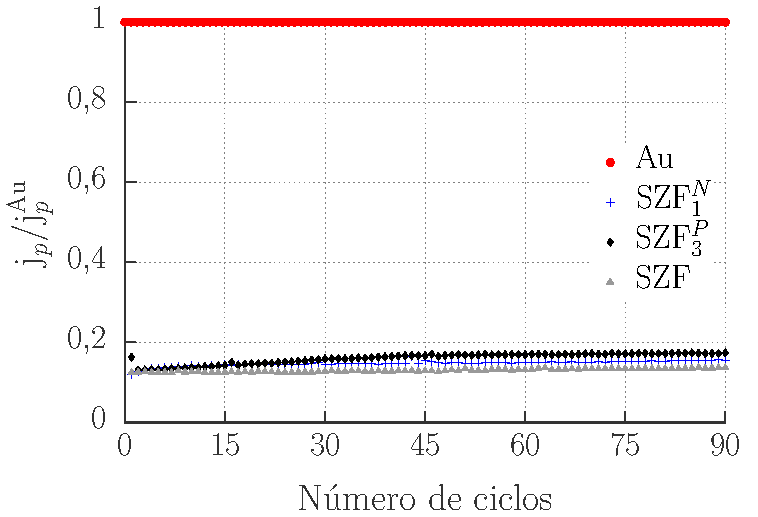
\includegraphics[width=\textwidth]{Graficos/ciclosintferroceno.pdf}
		      \end{subfigure}
			\begin{subfigure}[t]{0.495\textwidth}
		 	    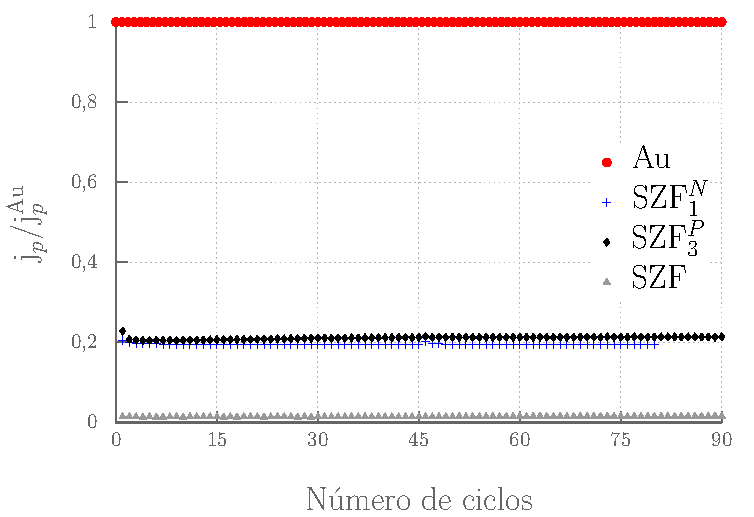
\includegraphics[width=\textwidth]{Graficos/ciclosintfecn.pdf}
			\end{subfigure}
		      	\caption[Corriente de pico de \fc\space y \fe\space en función del número de ciclos]{Corriente de pico anódico para \fc\space \SI{1}{\milli\Molar} (izquierda) y  \fe\space \SI{1}{\milli\Molar} (derecha) en función de la cantidad de ciclos. Los datos fueron tomados a una velocidad de barrido\index{velocidad!de barrido} de \SI{50}{\milli\volt\per\second} en solución de KCl \SI{100}{\milli\Molar} en un sensor\index{sensor} compuesto por cuatro electrodos diferentes: de Au\index{oro} (Au), recubierto con una pelicula mesoporosa\index{película!mesoporosa} sin funcionalizar\index{funcionalizar} (\pdmZ), con una funcionalizada con DHDP\index{dihexadecilfosfato} (\pdmZ$^P_3$) y con una funcionalizada con APTES\index{aminopropil@3-aminopropil trietoxisilano} (\pdmZ$^N_1$).}
		      	\label{fig:ciclos-fe-fcoh}
		      	\end{figure}
		     		
	Ya se estudió en detalle en el capítulo \ref{chap:Electrooquimica} la respuesta de los voltagramas para cada una de estas sonda\index{sonda}s. En el caso del \fe\space se tiene una fuerte exclusión por parte de las películas sin funcionalizar\index{funcionalizar} y una mínima permeación\index{permeacion} en las películas con APTES\index{aminopropil@3-aminopropil trietoxisilano} y DHDP\index{dihexadecilfosfato}. 
	En el caso del \fc\space en todos las casos el fenómeno dominante es la permeación, como es de esperar para una sonda\index{sonda} de carga neutra. Debido a que las membranas fueron condensadas y extraídas a bajas temperaturas la difusión\index{difusión} es lenta y la corriente resultante es bastante menor que la obtenida en electrodos de Au\index{electrodo!de Au} desnudo (consulta sección \ref{sec:difusion}, pág. \pageref{sec:difusion}). Las corriente de pico a lo largo de los ciclos para estas dos sonda\index{sonda}s es prácticamente invariante tal como se puede observar en los gráficos de la figura \ref{fig:ciclos-fe-fcoh}.

	El caso más interesante es de la sonda\index{sonda} positiva, el \ru. La intensidad de pico anódico, para condiciones de contorno constante (velocidad de barrido, pH\index{pH}, fuerza iónica, concentración de \ru\space en solución), evoluciona en cada ciclo de forma diferente según se va adsorbiendo en las películas delgadas mesoporosas. La interpretación de las distintas respuestas ya discutieron en la sección \ref{sub_sec_funcionalizaciones_chap_4}, pág. \pageref{sub_sec_funcionalizaciones_chap_4}. Al\index{aluminio} igual que para las otras sonda\index{sonda}s, en el gráfico \ref{fig:ruciclos}  se muestra como va cambiando la intensidad de pico, para cada electrodo, a medida que se aumenta la cantidad de ciclos electroquímico\index{electroquimico}s\index{electroquimico}. 

			\begin{figure}[ht!]
		 	       	\begin{center}
		 	       	\includegraphics[width=0.85\textwidth]{Graficos/ciclosintru.pdf}
		        	\caption[Corriente de pico de \ru\space en función del número de ciclos]{Corriente de pico anódico para \ru\space \SI{1}{\milli\Molar} en función de la cantidad de ciclos. Los datos fueron tomados a una velocidad de barrido\index{velocidad!de barrido} de \SI{50}{\milli\volt\per\second} en solución de KCl \SI{100}{\milli\Molar} en un sensor\index{sensor} compuesto por cuatro electrodos diferentes: de Au\index{oro} (Au), recubierto con una película mesoporosa\index{película!mesoporosa} sin funcionalizar\index{funcionalizar} (\pdmZ), con una funcionalizada con DHDP\index{dihexadecilfosfato} (\pdmZ$^P_3$) y con una funcionalizada con APTES\index{aminopropil@3-aminopropil trietoxisilano} (\pdmZ$^N_1$).}
		         	\label{fig:ruciclos}
		         	\end{center}
		     		\end{figure}
	
	Con el objetivo de utilizar los sensores\index{sensor} en aplicaciones analíticas se pueden sintetizar aún más los datos presentados en los gráficos \ref{fig:ciclos-fe-fcoh} y \ref{fig:ruciclos}. Durante la recolección de datos se pueden escoger aquellos que devuelve cada electrodo en un número de ciclo dado; luego se exponen estos resultados en un histograma como los que se muestra en la figura \ref{fig:barras}. En estos gráficos se volcaron los valores obtenidos en los ciclos 25 y 50 en cada uno de los cuatro electrodos diferentes, para cada una de los analitos electroactivos. De los histogramas se pueden establecer perfiles de respuestas para las sonda\index{sonda}s de concentración conocida, de forma que el sistema vaya almacenando las respuestas de cada electrodo en una base de datos, para luego comparar la respuesta de una muestra incógnita con la almacenada en la base. Mientras mayor sea la variabilidad de funcionalizaciones de las películas delgadas mesoporosas y la cantidad de electrodos diferentes por sensor, más inequívoca será identificación del analito, aún en matrices complejas, ya que la detección estará determinada por la respuesta de un conjunto de electrodos, limitado por las funcionalizaciones que se puedan llevar a cabo o por la cantidad de electrodos contemplada en el diseño.
   		

			\begin{figure}[h!]
		 	\begin{subfigure}[t]{0.495\textwidth}
		 	 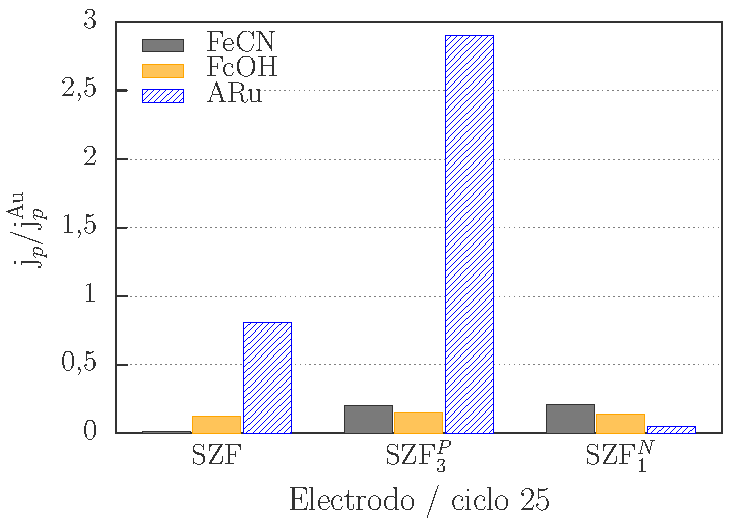
\includegraphics[width=\textwidth]{Graficos/histogramas-ciclo25.pdf}
		 	  \end{subfigure}
			\begin{subfigure}[t]{0.495\textwidth}
		 	   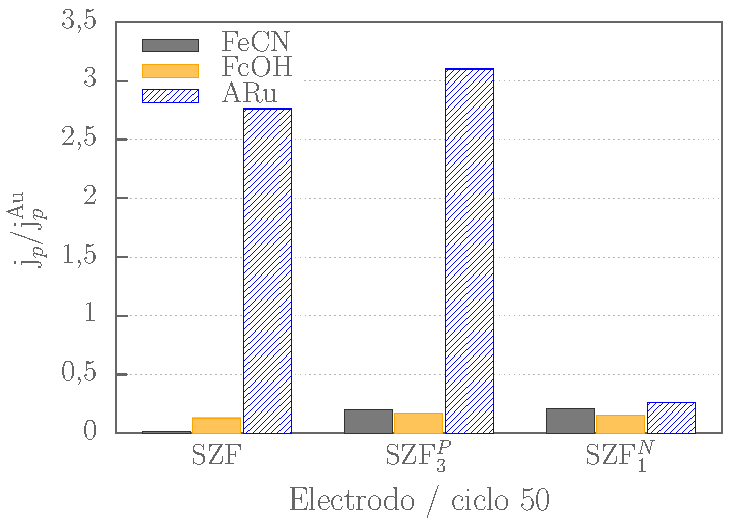
\includegraphics[width=\textwidth]{Graficos/histogramas-ciclo50.pdf}
		 	   \end{subfigure}
		      	\caption[Corriente de pico en distintos ciclos voltamperometricos]{Densidad de corriente anódica máxima en los ciclos 25 y 50 para cada uno de los electrodos del sensor. Las sonda\index{sonda}s probadas fueron \fc \SI{1}{\milli\Molar}, \fe\space \SI{1}{\milli\Molar} y \ru\space \SI{1}{\milli\Molar} en KCl \SI{100}{\milli\Molar} a una velocidad de barrido\index{velocidad!de barrido} de \SI{50}{\milli\volt\per\second}.}
		      	\label{fig:barras}
		      	\end{figure}

\section{Más allá de la microfabración}
	
	  Esta sección tiene por motivación mostrar y ejemplificar muy brevemente algunos experimentos, reflexiones y pruebas de concepto derivadas del presente trabajo. Estos experimentos generan nuevas incógnitas y abren líneas de investigación y desarrollo en el área de sensores. No es el propósito de este apartado realizar demostraciones formales o hacer discusiones profundas de los resultados, sino mostrar los avances y conceptos surgidos de los conocimientos y experiencia adquieridas durante esta tesis con perspectivas a futuros desarrollos e investigaciones.

	\subsection{Integración en microchips de silicio}

	  La ventaja de fabricar electrodos por técnicas de microelectrónica\index{microelectrónica} es indiscutible. Hay muchas fabricas a nivel global de microsistemas (MEMS\index{MEMS}) y circuitos integrados (IC) (conocidas en ingles simplemente como \textit{foundry}\index{foundry@\textit{foundry}}). Dichas fabricadas elaboran sus productos con procesos estándar de fabricación, por cada nodo tecnológico, con reglas de diseño claras, rígidas y bien establecidas. La integración de sensores\index{sensor} en circuitos integrados no es algo nuevo, y, dado el nivel de integración de la electrón\index{electrón}ica de las últimas décadas, es algo que siempre se debe tener en cuenta en la etapa de prototipado de sensores.\cite{Wang2012,Liu1993,Novell2012,Yu2013,Sarkar2014} Debido al desarrollo y optimización de los procesos para depositar \pdm\space a bajas temperaturas se podría fácilmente integrar los sensores\index{sensor} EQ en un solo chip\index{chip} con potenciostato\index{potenciostato} integrado en la lógica del IC.
 	
 	\subsection{Sensores y electrodos flexibles e impresos}

 	  Se realizaron pruebas conceptuales sobre impresión de mesoporosos, con el objetivo de realizar cualquier diseño arbitrario en la película mesoporosas. Se usaron los soles\index{sol} como tintas\index{tintas} y se imprimieron sobre diversos sustratos, además, de esta forma se podrían imprimir \pdm\space de igual o distintos óxidos en un mismo sustrato. Se trabajó en colaboración con el grupo del Dr. Baumann\index{Baumann}, del \textit{Department of Digital Printing and Imaging Technology} de la \textit{Technische Universität Chemnitz} de Al\index{aluminio}emania (\url{https://www.tu-chemnitz.de/mb/DigiTech/professorship.php}). Al\index{aluminio}lí imprimieron soles\index{sol} modificados con etilenglicol\index{etilenglicol}l con un equipo de inyección de tinta\index{inyección de tinta}. Los procesos a baja temperatura desarrollos en este trabajo, no solo hacen que disminuya la difusión\index{difusión} entre las capas metálicas, permitiendo la integración en chip\index{chip}s de silicio, sino que permite depositar las \pdm\space sobre sustratos térmicamente menos estables. Los resultados fueron sistemas porosos de soles\index{sol} de SiO$_2$, estructurados con F127 impresos sobre silicio, oro, microelectrodo\index{electrodo!microelectrodo}s y poliestireno\index{poliestireno} de alto impacto (PAI). Se muestran, en la figura \ref{fig:flexibles}, patrones cuadrados impresos sobre una diversidad de sustratos variando los parámetros de impresión, con el objetivo de encontrar las condiciones óptimas para una correcta transferencia.

 		%imagenes Meso en Au, Meso en Silicio, Meso en Au\index{oro} con patrones, SEM
 	  		\begin{figure}[th]
			 	   	    \centering
			 	   	    \begin{subfigure}[t]{0.495\textwidth}
			        	\includegraphics[width=\textwidth]{Imagenes/Inkjet-02-escala-fondo.jpg}
			        	\caption{\pdmF\space impresos sobre oblea\index{oblea} de silicio.}
			       		\end{subfigure}
			     		\centering
			     		\begin{subfigure}[t]{0.495\textwidth}
			     		\includegraphics[width=0.85\textwidth]{Imagenes/Inkjet-05-escala-fondo.jpg}
			    		\caption{\pdmF\space impresos sobre oblea\index{oblea} de silicio\index{silicio} con un depósito\index{depósito} de Ti\index{titanio}\textbar Au.}
			    		\end{subfigure}
			    		\centering
			    		\begin{subfigure}[t]{0.495\textwidth}
			         	\includegraphics[width=0.80\textwidth]{Imagenes/Inkjet-04-escala-fondo.jpg}
			        	\caption{\pdmF\space impresos sobre microelectrodo\index{electrodo!microelectrodo}s.}
			        	\end{subfigure}
			        	\centering
			        	\begin{subfigure}[t]{0.495\textwidth}
			     		\includegraphics[width=\textwidth]{Imagenes/Inkjet-03-escala-fondo.jpg}
 			        	\caption{\pdmF\space impresos en Ti\index{titanio}\textbar	Au en soporte de poliestireno\index{poliestireno} de alto impacto.}
			        	\end{subfigure}
			     		\caption[Electrodos impresos]{Fotografías de patrones impresos de óxido de silicio\index{silicio!oxido de}\index{silicio} mesoporoso por inyección de tinta\index{inyección de tinta}. Los poros fueron moldeados con F127 y la condensación\index{condensación} se realizó por el método de alto vacío\index{alto@alto vacío}. La extracción\index{extracción} se llevó a cabo con 2-propanol\index{propanol@2-propanol} y agua\index{agua}.}
			     		\label{fig:flexibles}
			     	   	\end{figure}
			     	  
 	  Con la expectativa de poder realizar todo el proceso de fabricación de los sensores\index{sensor} con técnicas de impresión, se muestran en la figura \ref{fig:tintas}, electrodos impresos por inyección con tintas\index{tintas} a base a nanotubos de carbono\index{nanotubos de carbono} desarrolladas en el INTI\index{INTI}-CMNB. Actualmente estas tintas\index{tintas} están en desarrollo y en proceso de optimización para uso en sensores\index{sensor} EQ y enzimáticos\cite{longinotti2010,Mass2016}. En la figura \ref{fig:tintas} también se muestra la respuesta EQ para \fe\space \SI{2.5}{\nm}, si bien no es la misma que en electrodos de Au\index{electrodo!de Au}, es una respuesta reproducible y confiable. Se prevé próximamente imprimir ambos componentes en un solo sustrato, los electrodos y películas delgadas mesoporosos.

 	  	%imagenes flexo + voltagrama
 	  			\begin{figure}[th]
		 	   	    \begin{subfigure}[t]{0.25\textwidth}
			       	\includegraphics[width=\textwidth]{Imagenes/NTC1-fondo.jpg}
			   		\end{subfigure}
			   		\begin{subfigure}[t]{0.25\textwidth}
			       	\includegraphics[width=\textwidth]{Imagenes/NTC2-fondo.jpg}
			   		\end{subfigure}
			   		\begin{subfigure}[t]{0.43\textwidth}
			   	    \includegraphics[width=\textwidth]{Graficos/TintaNTC-FeCN2-5mM.pdf}
			   		\end{subfigure}
					 \caption[Electrodos de NTC flexibles.]{Electrodos impresos por inyección de tinta\index{inyección de tinta} en base a nanotubos de carbono\index{nanotubos de carbono} donde se muestra la flexibilidad de la tinta y su respuesta electroquímica\index{electroquimico} con una sonda\index{sonda} de \fe\space \SI{2.5}{\milli\Molar} en solución de KCl \SI{100}{\milli\Molar} a \SI{50}{\milli\volt\per\second}.}
					 \label{fig:tintas}	
				     \end{figure}
 
\section{Conclusiones parciales}

	Se presentaron en este capítulo los resultados obtenidos durante el proceso de fabricación de los sensores. Se idearon dos diseños, de los cuales el segundo (retroalimentado de la experiencia del primero) es más compacto, incorpora más electrodos por sensor\index{sensor} y prevé el uso de contraeletrodo y referencia integrados en el mismo dispositivo.
	
	Los mismos fueron fabricados por un conjunto de técnicas conocidas como \textit{top-down}\index{top-down@\textit{top-down}}, propios de la microelectrónica\index{microelectrónica} como: fotolitografía\index{fotolitografía} óptica, deposición por pulverización catódica\index{pulverización catódica} y \textit{lift-off}\index{lift@\textit{lift-off}}, entre otras. Se establecieron las condiciones óptimas de proceso para cada etapa, y, una vez conseguido resultados satisfactorios, se evaluó el desempeño electroquímico\index{electroquimico} de los sensores, el cuál resulto óptimo. 

	Sobre los electrodos de (Ti,Cr)\textbar Au\index{oro} se realizaron los primeros depósitos de películas delgadas mesoporosas de sílice. En esta etapa surgieron algunas dificultades, en particular, en lo referente al sensado electroquímico\index{electroquimico}. Se realizó un estudio meticuloso sobre la superficie\index{superficie} de los electrodos.  Se discutió como se vió afectado el desempeño electroquímico\index{electroquimico} durante los procesos de calcinación\index{calcinación} debido a fenómenos de difusión\index{difusión} de interferentes hacia la superficie\index{superficie} de lo electrodos, afectando sensiblemente la trasferencia de carga entre la sonda\index{sonda} y el electrodo. 

	Éste fue uno de los motivos (junto con con otros como utilizar polímeros, evitar calcinaciones y reducir costos) para el desarrollo de procesos de síntesis de películas mesoporosas de SiO$_2$ a temperaturas menores que las clásicas de calcinación\index{calcinación}, donde se minimizan los procesos difusivos y no es necesario recurrir a metales de ultra pureza. Las consecuencias directas de este desarrollo fueron que se pudo depositar los óxidos sobre Au\index{oro} metalúrgico (Au3N) sin perder desempeño analítico y, a su vez, permitió depositar las \pdm\space sobre sustratos que sean estables a \SI{130}{\celsius}. Dicho desarrollo se estudia extensamente en el capítulo \ref{chap:Mesoporosos}, mientras que en el capítulo \ref{chap:Electroquimica} se estudia la estabilidad química y mecánica de la películas sintetizadas.

	Ya con el proceso de síntesis optimizado se escogieron las películas más estables para la fabricación de un sensor\index{sensor} prototipo. Se fabricaron nuevamente electrodos con el diseño en forma de calesita y se depositaron sobre ellas películas mesoporosas de Si$_{0.9}$Zr$_{0.1}$O$_2$ mediante el método de alto vacío\index{alto@alto vacío}. Sobre uno de los sensores\index{sensor} se funcionalizar\index{funcionalizar}on estás películas porosas con dihexadecilfosfato\index{dihexadecilfosfato} (DHDP) y 3-aminopropil trietoxisilano (APTES\index{aminopropil@3-aminopropil trietoxisilano}), específicamente sobre el área de cada electrodo.
	Se analizaron las respuestas amperométrica de cada electrodo de este sensor\index{sensor} en función del ciclado electroquímico\index{electroquimico}, obteniéndose patrones de respuesta para cada una de las sonda\index{sonda}s en función de la interacción entre la sonda\index{sonda} y la película. 
	
	Finalmente se exploraron algunas técnicas de depósito\index{depósito} mediante impresión por inyección de tinta\index{inyección de tinta} con el objetivo de poder transferir algún diseño a las películas mesoporosas.























	